% Provenance (never printed): old terminale S material on the early Earth (the
% primitive atmosphere and its outgassing, the first traces of life, the rise of
% oxygen read in the rocks: banded iron formations, red beds) and the faint young
% Sun. Owner (Sync 0/1): outgassing and primitive atmosphere, faint young Sun
% problem, stromatolite, Great Oxidation Event, banded iron formation, red beds.
% Recalled: age of the Earth (g12.07), zircons (g12.01), equilibrium temperature
% (g10.02), photosynthesis and cyanobacteria (biology), air composition, greenhouse
% gases as molecules and redox (chemistry). Figures: figdata/grade-12/early_earth.py.
\chapter{早期地球及其大气}\label{ch:g12:early-earth}

在澳大利亚西北部的哈默斯利山脉中，戴尔斯峡谷
的岩壁像层叠的蛋糕一样呈条纹状：红色、灰色和黑色的薄层岩石交错排列。
这是一种\omterm{def:g12:early-earth:bif}{条带状铁建造}，形成于 25 亿多年
前的海底。
其中的铁在那片海中生锈，而生锈需要氧气。
本章探讨年轻的地球及其大气是怎样的，
以及岩石如何记录氧气出现的那一刻。
% ledger: dbca:karijini, earle:bif, photo:g12-dales-gorge

\begin{omfigure}
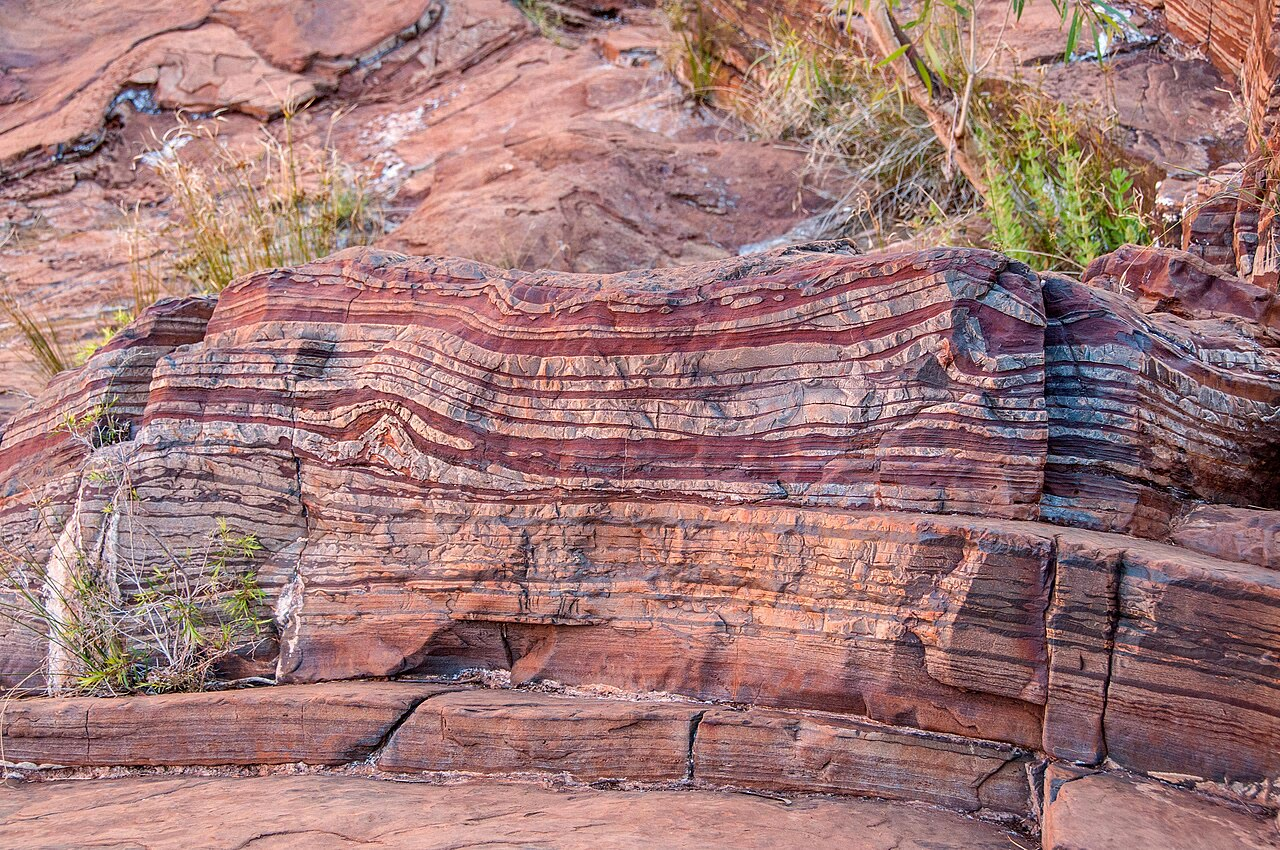
\includegraphics[width=0.72\linewidth]{images/book2/g12-dales-gorge-bif.jpg}

{\small \omterm{def:g12:early-earth:bif}{条带状铁建造}，位于西澳大利亚卡里吉尼国家公园
戴尔斯峡谷的福蒂斯丘瀑布。照片：Graeme Churchard, CC~BY~2.0
（维基共享资源）。}
\end{omfigure}

\begin{recall}
地球的年龄为 45.4 亿年（见\cref{ch:g12:age-of-the-earth}），
锆石表明地壳早在 44 亿年前就已存在（见\cref{ch:g12:continental-crust}）。
行星的\omterm{def:g10:habitable-planet:equilibrium-temperature}{平衡温度}，
$T_{\mathrm{eq}} = \left(S(1-A)/(4\sigma)\right)^{1/4}$，今日地球的\omterm{def:g10:habitable-planet:equilibrium-temperature}{平衡温度}约为 \qty{255}{K}
（见\cref{ch:g10:habitable-planet}）。今日干燥空气中，氮气约占
\qty{78}{\percent}，氧气约占 \qty{21}{\percent}，二氧化碳和甲烷
是温室气体；能与氧结合的元素会被氧化（见化学书籍）。
植物、藻类和蓝细菌借助光合作用制造食物，
这一过程释放氧气（见生物书籍）。
\end{recall}
% ledger: usgs:age-earth (Book 1 row), wilde01:zircon, earth:TSI, earth:albedo, air:N2, air:O2

\section{年轻的地球}

地球由较小天体吸积而增长。太阳系开始形成后约
6000 万年后，一个大小可能与火星相当的天体撞击了地球，
被抛入太空的物质形成了月球。年轻的地球
炽热且仍\omterm{def:g11:ocean-ridges:partial-melting}{部分熔融}。它逐渐冷却，到约 44 亿年前
已形成地壳和海洋：那个年代的锆石带有
液态水的化学印记。
% ledger: nasa:moon-formation, wilde01:zircon

\section{原始大气}

\begin{definition}[脱气；原始大气]\label{def:g12:early-earth:primitive-atmosphere}
\emph{脱气}\index{脱气}是由火山和地面
释放岩浆中溶解气体的过程。\emph{原始
大气}\index{原始大气}是生物改变之前的地球大气，
主要由脱气形成，含有氮气、二氧化碳和水蒸气，
二氧化碳含量比今天更高，
几乎不含游离氧。
\end{definition}
% ledger: usgs:volcanic-gases (Book 1 row), holland06:stages (stage 1 anoxic), feulner12:fys (more carbon dioxide)

火山活动今天仍能说明这类大气如何形成：岩浆上升、
压强降低时，溶解的气体逸出，其中数量最多的是
水蒸气，其次是二氧化碳。氮气和二氧化碳，这两种
曾在原始空气中占主导的气体，至今仍是火山
喷出的主要含氮、含碳气体。水蒸气凝结成了
海洋。此时的氧气含量
不足今天大气水平的 \qty{0.001}{\percent}。
% ledger: usgs:volcanic-gases (Book 1 row), pk02:anoxic

年轻的太阳比今天暗淡。太阳核心中氢转变为
氦，核心收缩并升温，太阳的功率
缓慢上升。

\begin{proposition}[年轻太阳的光度]\label{prop:g12:early-earth:luminosity}
记太阳的现龄为 $t_\odot$，现在的光度为 $L_\odot$，
则太阳年龄为 $t$ 年时的光度为
\[
  L(t) = \frac{L_\odot}{1 + \frac{2}{5}\left(1 - t/t_\odot\right)} .
\]
\end{proposition}
% ledger: gough81:luminosity, connelly12:cai

这一对太阳计算模型的近似在本阶段不加证明地承认。在
太阳诞生时，$t = 0$，由此得 $L = L_\odot/1.4 \approx 0.71\,L_\odot$：
年轻的太阳约暗 \qty{30}{\percent}。

\begin{example}[40 亿年前的地球]\label{ex:g12:early-earth:young-sun}
取 $t_\odot = 4.567$（单位：十亿年）。40 亿年前，太阳
的年龄为 5.67 亿年，故 $1 - t/t_\odot = 4/4.567 \approx 0.876$，且
$L \approx L_\odot/1.350 \approx 0.741\,L_\odot$。到达地球的太阳辐射
为 $0.741 \times 1361 \approx \qty{1008}{W/m^2}$。保持今天的
\omterm{def:g10:earth-energy-budget:albedo}{反照率}不变，\omterm{def:g10:habitable-planet:equilibrium-temperature}{平衡温度}与太阳辐射的四次方根成正比：
$255 \times 0.741^{1/4} \approx 255 \times 0.928 \approx
\qty{237}{K}$，约 \qty{-36}{\celsius}。
\end{example}
% values: L_4Ga 0.7406, S_4Ga 1007.9, Teq_today 255.1, Teq_4Ga 236.7 (early_earth.py)

\begin{omfigure}
\begin{tikzpicture}
\begin{axis}[omrecord, scale only axis, width=0.66\linewidth, height=4.6cm,
  xmin=0, xmax=4.6, ymin=225, ymax=295, x dir=reverse, axis y line*=left,
  xlabel={距今时间（十亿年）}, ylabel={温度（K）},
  xtick={0,0.5,...,4.5}, x tick label style={/pgf/number format/.cd, fixed, precision=1}]
% computed in figdata/grade-12/early_earth.py; ledger: gough81:luminosity, earth:TSI, earth:albedo, earth:Tsurf
\addplot[omDef, line width=1.2pt] table[x=t_Ga, y=Teq] {figdata/out/grade-12-early_earth-sun.dat};
\addplot[omThm, densely dashed, domain=0:4.6, samples=2] {273.15};
\addplot[black!60, densely dotted, domain=0:4.6, samples=2] {288};
\coordinate (teq) at (axis cs:2.6,239);
\coordinate (frz) at (axis cs:2.3,274);
\coordinate (sfc) at (axis cs:2.3,289);
\end{axis}
\begin{axis}[omrecord, scale only axis, width=0.66\linewidth, height=4.6cm,
  xmin=0, xmax=4.6, ymin=0.65, ymax=1.05, x dir=reverse, axis y line*=right, axis x line=none,
  ylabel={太阳光度（$L_\odot$）}, ymajorgrids=false, xmajorgrids=false,
  y tick label style={/pgf/number format/.cd, fixed, fixed zerofill, precision=2}]
\addplot[omProp, line width=0.9pt, densely dashdotted] table[x=t_Ga, y=L] {figdata/out/grade-12-early_earth-sun.dat};
\coordinate (lum) at (axis cs:1.7,0.86);
\end{axis}
\node[font=\scriptsize, text=omDef, anchor=north] at (teq) {平衡温度};
\node[font=\scriptsize, text=omThm, anchor=south] at (frz) {水凝固，\qty{273}{K}};
\node[font=\scriptsize, text=black!70, anchor=south] at (sfc) {今日地表平均温度，\qty{288}{K}};
\node[font=\scriptsize, text=omProp, anchor=north west] at (lum) {光度（右侧刻度）};
\end{tikzpicture}

{\small 黯淡的年轻太阳：其光度（右侧刻度）与地球的
\omterm{def:g10:habitable-planet:equilibrium-temperature}{平衡温度}（取今日\omterm{def:g10:earth-energy-budget:albedo}{反照率}，左侧刻度），回溯至太阳诞生之时。
依今日的日光与\omterm{def:g10:earth-energy-budget:albedo}{反照率}，由 Gough（1981）计算得出。}
\end{omfigure}

\begin{definition}[黯淡太阳悖论]\label{def:g12:early-earth:faint-young-sun}
\emph{黯淡太阳悖论}\index{黯淡太阳悖论}是指
地球最初数十亿年间较暗淡的太阳（在此太阳下，
若大气与今日相同，地球本会冻结）与岩石显示
当时存在液态水之间的矛盾。
\end{definition}
% ledger: feulner12:fys

1972 年，卡尔·萨根与乔治·穆伦使这一问题广为人知，
二人提出以更强的温室效应作答。此后研究的答案大多依赖
\omterm{def:g12:early-earth:primitive-atmosphere}{原始大气}中更多的温室气体：
二氧化碳含量远高于今日、早期微生物产生的甲烷，或
二者兼有。在一个经典计算中，约十分之一巴的二氧化碳，
再加少量甲烷，即可使早期地球与今日同样温暖；若无甲烷，
则需约三倍的二氧化碳。该问题尚未
被视为已解决。
% ledger: feulner12:fys

\section{生命与氧气}

\omterm{def:g12:early-earth:stromatolite}{叠层石}的化石记录覆盖了近 35 亿年：
它们是最古老的生命迹象之一。

\begin{definition}[叠层石]\label{def:g12:early-earth:stromatolite}
\emph{叠层石}\index{叠层石}是一种成层的丘状体，由以蓝细菌为主的
微生物席在浅水中建造：微生物席捕获并黏结沉积物颗粒，
使碳酸盐逐层生长。
\end{definition}
% ledger: noffke13:stromatolites

距今 34.3 亿年的\omterm{def:g12:early-earth:stromatolite}{叠层石}化石，见于西澳大利亚皮尔巴拉
的 Strelley Pool Chert 地层。现今仍有活体\omterm{def:g12:early-earth:stromatolite}{叠层石}生长于
鲨鱼湾的哈默林池，这里的海水盐度是
通常海水的两倍，是现代最著名的例子。
% ledger: allwood06:spc, noffke13:stromatolites, dbca:hamelin

\begin{omfigure}
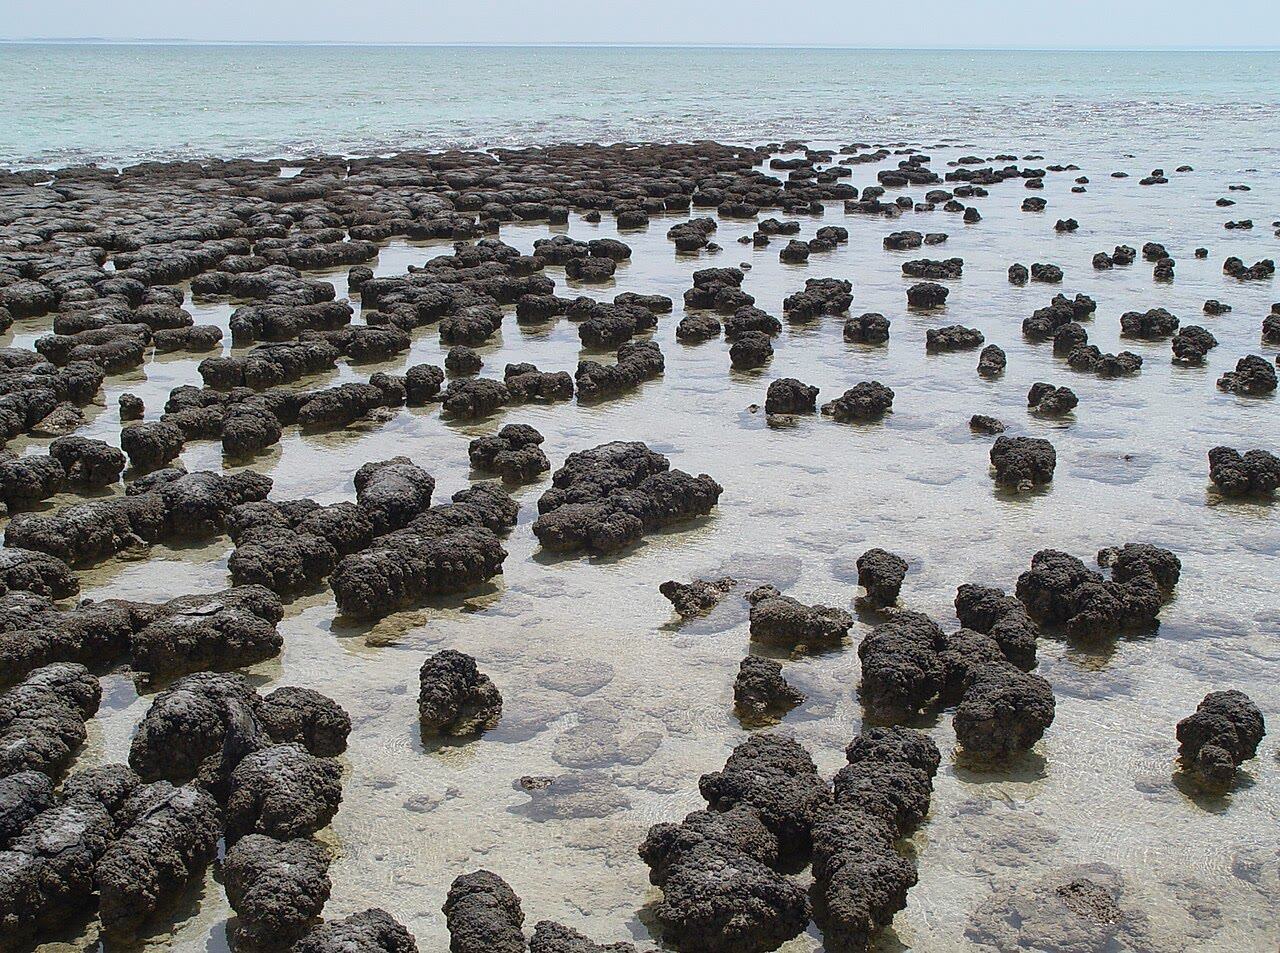
\includegraphics[width=0.6\linewidth]{images/book2/g12-shark-bay-stromatolites.jpg}

{\small 西澳大利亚鲨鱼湾哈默林池中的活体\omterm{def:g12:early-earth:stromatolite}{叠层石}。
照片：Paul Harrison, CC~BY-SA~3.0（维基共享资源）。}
\end{omfigure}
% ledger: photo:g12-shark-bay

蓝细菌带来了新事物：一种释放氧气的
光合作用。但很长时间里，它们产生的氧气并未留在空气中，
产生后随即被消耗：被海水中溶解的铁、
硫和甲烷消耗殆尽。

\section{氧气的兴起}

在氧气出现之前，铁以溶解于海水中的离子
\ce{Fe^2+} 形式迁移。氧气将其氧化为三价铁，三价铁不溶解：
它会沉降至海底，形成锈色沉积物。

\begin{proposition}[铁消耗氧气]\label{prop:g12:early-earth:iron}
溶解的二价铁被水中的氧气氧化为氢氧化三价铁，
并沉淀析出：
\[
  \ce{4Fe^2+ + O2 + 10H2O -> 4Fe(OH)3 + 8H+} .
\]
每个氧分子可去除四个溶解的铁离子；只要
溶解的铁尚存，产生的氧气便被消耗殆尽。
\end{proposition}
% ledger: earle:bif (ferrous iron oxidised to insoluble ferric iron)

\begin{proof}
检验配平。铁：两边各为 4。氧：左侧 $2 + 10 = 12$，
右侧 $4 \times 3 = 12$。氢：左侧 $20$，右侧 $4 \times 3 + 8 =
20$。电荷：左侧 $4 \times (+2) = +8$，右侧 $8 \times (+1) =
+8$。
\end{proof}

\begin{definition}[条带状铁建造]\label{def:g12:early-earth:bif}
\emph{条带状铁建造}\index{条带状铁建造}是一种沉积岩，
由薄层交替排列的铁氧化物（如赤铁矿）与
燧石（贫铁的细粒二氧化硅）组成，几乎全部
形成于 18 亿年以前。
\end{definition}
% ledger: earle:bif, holland06:stages

\omterm{def:g12:early-earth:bif}{条带状铁建造}需要两种水体同时存在：缺氧的\omterm{def:g10:layered-ocean:thermocline}{深海}，
携带溶解的铁；以及浅层的、有阳光照射的海域，蓝细菌在其中
产生氧气，铁在此沉淀。此类岩层常见于距今 24 亿至
18 亿年的岩石中，哈默斯利山脉的此类岩层更为古老。
\omterm{def:g12:early-earth:bif}{条带状铁建造}是常见的铁矿石。
% ledger: earle:bif, holland06:stages (Archean BIF, Hamersley), dbca:karijini

\begin{omfigure}
\begin{tikzpicture}[x=1cm, y=1cm, font=\scriptsize]
  % sea and floor
  \fill[omSea] (0,0) rectangle (11,4);
  \fill[omSea!45!white] (0,2.9) rectangle (11,4);
  \draw[omDef!60, line width=0.4pt, densely dashed] (0,2.9) -- (11,2.9);
  \node[anchor=north east, text=omDef] at (10.9,3.95) {阳光照射的表层水};
  \node[anchor=south east, text=omDef, align=right] at (10.9,0.12) {深层水体 \\缺氧，\\富含 \ce{Fe^2+}};
  % floor with layers
  \foreach \i/\c in {0/red!55!black, 1/black!20, 2/red!55!black, 3/black!20, 4/red!55!black, 5/black!20} {
    \fill[\c] (0,-0.12*\i) rectangle (11,-0.12*\i-0.12);
  }
  \draw[black!60] (0,0) -- (11,0);
  \node[anchor=west] at (11.1,-0.12) {铁氧化物};
  \node[anchor=west] at (11.1,-0.36) {燧石};
  \draw[black!50, line width=0.3pt] (11.05,-0.06) -- (10.6,-0.06);
  \draw[black!50, line width=0.3pt] (11.05,-0.30) -- (10.6,-0.30);
  % upwelling iron
  \foreach \x in {0.5,1.0,1.5} {
    \draw[-{Stealth}, omDef, line width=0.8pt] (\x,0.4) .. controls (\x+0.4,1.5) and (\x+0.6,2.2) .. (\x+0.9,2.85);
  }
  \node[text=omDef, anchor=west] at (2.3,1.3) {\ce{Fe^2+} 上升};
  % cyanobacteria and oxygen
  \foreach \x in {3.8,4.4,5.0,5.6,6.2} {\fill[green!45!black] (\x,3.35) circle (0.07);}
  \node[anchor=south, text=green!35!black] at (5.0,3.47) {蓝细菌产生 \ce{O2}};
  % reaction
  \node[draw=black!40, fill=white, rounded corners=2pt, inner sep=2pt] at (5.4,2.45) {\ce{4Fe^2+ + O2 + 10H2O -> 4Fe(OH)3 + 8H+}};
  % falling rust
  \foreach \x/\y in {4.6/1.9, 5.0/1.5, 5.5/1.8, 5.9/1.2, 4.3/1.1, 5.2/0.7, 6.1/0.6} {\fill[red!60!black] (\x,\y) circle (0.06);}
  \draw[-{Stealth}, red!60!black, line width=0.6pt] (6.6,2.1) -- (6.6,0.25);
  \node[anchor=west, text=red!60!black, align=left] at (6.7,1.75) {三价铁沉降 \\形成锈色层};
\end{tikzpicture}

{\small \omterm{def:g12:early-earth:bif}{条带状铁建造}的形成过程（示意图，未按比例）：铁
溶解于不含氧气的深水中，上升进入阳光照射的海面，
在蓝细菌产生的氧气作用下转化为三价铁，
三价铁沉降。富铁层与燧石层交替出现。}
\end{omfigure}

此后，氧气开始在大气中留存。

\begin{definition}[大氧化事件]\label{def:g12:early-earth:goe}
\emph{大氧化事件}\index{大氧化事件}是指
约 \num{2.46} 十亿年前至约 \num{2.06} 十亿年前这段时间内，
自由氧首次在地球大气和浅海中积累，
达到现今水平的约十分之一。
\end{definition}
% ledger: gumsley17:goe, holland06:stages (0.02-0.04 atm, about a tenth of 0.21)

证据保存在岩石中。部分矿物（其中包括黄铁矿和沥青铀矿）
会被氧气破坏；然而其颗粒经河流搬运后，
仍见于古老沉积物中；而在氧气上升之后沉积的地层中，
则见不到黄铁矿颗粒。早于 2.45 十亿年的岩石中的硫同位素，
带有一种特征，只有氧气含量不足今日十万分之一的大气才能留下；
到 2.09 十亿年前，这一特征已经消失。此外，陆地上出现了
\omterm{def:g12:early-earth:red-beds}{红层}。
% ledger: kasting25:indicators, pk02:anoxic, farquhar00:sulfur

\begin{definition}[红层]\label{def:g12:early-earth:red-beds}
\emph{红层}\index{红层}是沉积岩——砂岩、
粉砂岩、页岩——因颗粒外包裹三氧化二铁而呈红色，
即赤铁矿，附着于颗粒上。它们只形成于有足够氧气
使铁氧化的地方。
\end{definition}
% ledger: kasting25:indicators (redbeds an oxygen indicator)

\begin{omfigure}
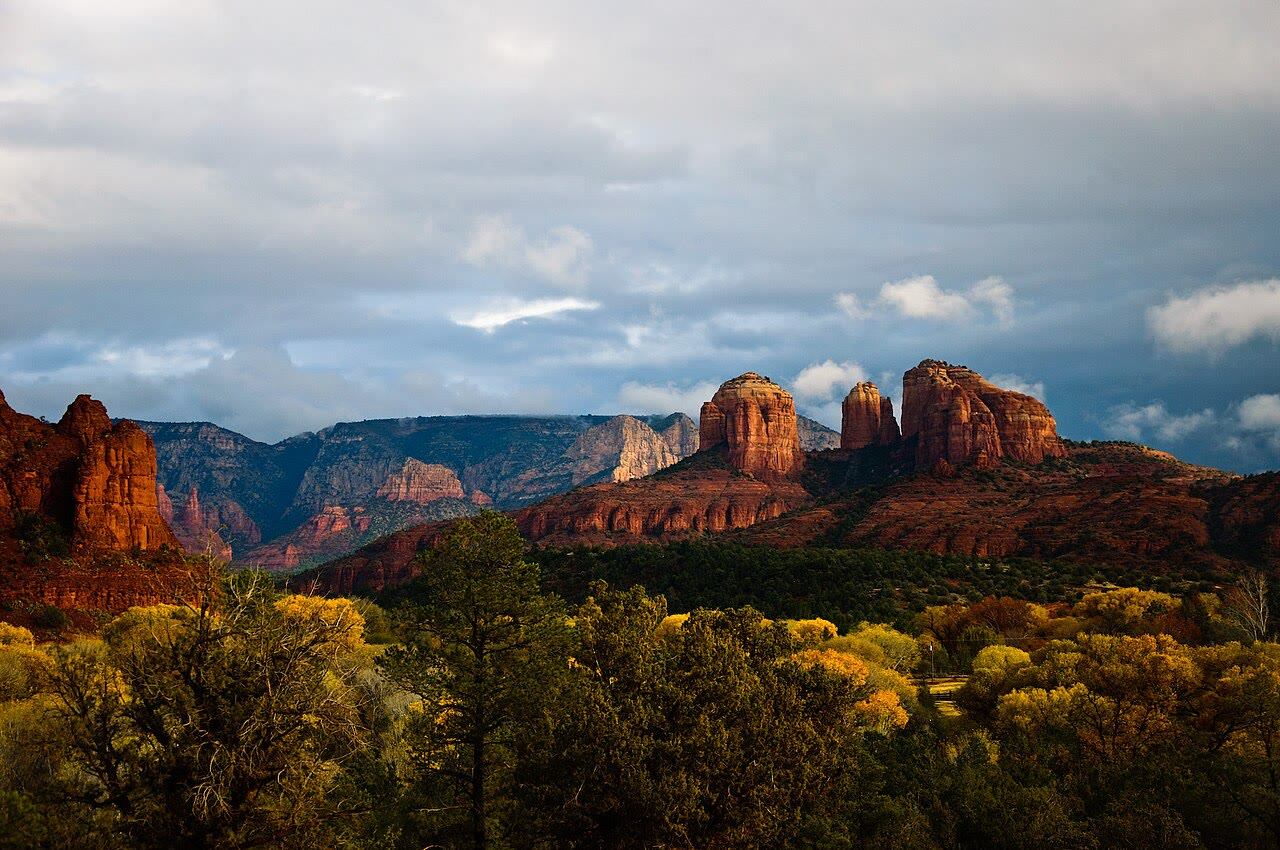
\includegraphics[width=0.66\linewidth]{images/book2/g12-sedona-red-beds.jpg}

{\small \omterm{def:g12:early-earth:red-beds}{红层}：亚利桑那州塞多纳附近的大教堂岩，由二叠纪红色
砂岩构成。照片：Wendy from Pennsylvania, CC~BY-SA~2.0，
维基共享资源。}
\end{omfigure}
% ledger: photo:g12-sedona, azgs:cathedral (Permian Schnebly Hill Sandstone)

\omterm{def:g12:early-earth:bif}{条带状铁建造}的形成基本在 1.8 十亿年前停止：到那时，
\omterm{def:g10:layered-ocean:thermocline}{深海}中也已有足够氧气，使其不再能携带铁。
此后的十亿年间，氧气含量变化不大；0.85 十亿年前之后，氧气含量再次升高，
逐渐接近今日的 \qty{21}{\percent}。
% ledger: earle:bif, holland06:stages

\begin{method}[读取地质时间线]\label{met:g12:early-earth:timeline}
\begin{enumerate}
  \item 确定坐标轴上时间的方向及其单位（
        以百万年或十亿年前计）。
  \item 在彩色色带上找出各宙，并读出其界限。
  \item 对每一事件，读出其发生的时间或时间区间，
        并说明是何种记录给出了该时间（矿物、化石或岩石）。
  \item 通过减法计算各时长，并将其与
        \omterm{def:g12:age-of-the-earth:age}{地球年龄}进行比较。
  \item 检查先后顺序：结果不能早于其原因。
\end{enumerate}
\end{method}

\begin{omfigure}
\begin{tikzpicture}
\begin{axis}[omrecord, width=0.82\linewidth, height=6.2cm, ymode=log, xmin=0, xmax=4.6, ymin=1e-7, ymax=5,
  x dir=reverse, xlabel={距今时间（十亿年）}, ylabel={大气中的氧气（今日 $=1$）},
  xtick={0,0.5,...,4.5}, x tick label style={/pgf/number format/.cd, fixed, precision=1},
  ytick={1e-6,1e-4,1e-2,1}, ymajorgrids=true, xmajorgrids=false, clip=false]
% computed in figdata/grade-12/early_earth.py (schematic through the sourced bounds); ledger: holland06:stages, pk02:anoxic, gumsley17:goe, ics:base.Hadean, ics:base.Archean, ics:base.Proterozoic, ics:base.Paleozoic
\fill[omThm!12] (axis cs:2.46,1e-7) rectangle (axis cs:2.06,5);
\addplot[black, line width=1.2pt] table[x=t_Ga, y=pal] {figdata/out/grade-12-early_earth-oxygen.dat};
% eon band (ICS colours), below the axis
\fill[icsHadean] (axis cs:4.567,1.5e-7) rectangle (axis cs:4.031,4e-7);
\fill[icsArchean] (axis cs:4.031,1.5e-7) rectangle (axis cs:2.5,4e-7);
\fill[icsProterozoic] (axis cs:2.5,1.5e-7) rectangle (axis cs:0.5388,4e-7);
\fill[icsPhanerozoic] (axis cs:0.5388,1.5e-7) rectangle (axis cs:0,4e-7);
\node[font=\tiny, text=white] at (axis cs:4.30,2.45e-7) {冥古宙};
\node[font=\tiny, text=white] at (axis cs:3.27,2.45e-7) {太古宙};
\node[font=\tiny, text=white] at (axis cs:1.52,2.45e-7) {元古宙};
% events
\draw[omDef, line width=0.6pt] (axis cs:4.4,4e-7) -- (axis cs:4.4,3e-3);
\node[font=\scriptsize, text=omDef, anchor=south west] at (axis cs:4.4,3e-3) {锆石、水};
\draw[omMeth, line width=0.6pt] (axis cs:3.43,4e-7) -- (axis cs:3.43,1.2e-6);
\node[font=\scriptsize, text=omMeth, anchor=south] at (axis cs:3.43,1.2e-6) {最早的叠层石};
\draw[red!60!black, line width=3pt] (axis cs:2.4,3e-6) -- (axis cs:1.8,3e-6);
\node[font=\scriptsize, text=red!60!black, anchor=north] at (axis cs:2.16,2.4e-6) {条带状铁建造};
\node[font=\scriptsize, text=omThm, anchor=south, align=center] at (axis cs:2.26,1.2) {大氧化 \\事件};
\node[font=\scriptsize, anchor=south] at (axis cs:3.2,1.3e-5) {今日的 $10^{-5}$ 以下};
\node[font=\scriptsize, anchor=south] at (axis cs:1.4,0.12) {约十分之一};
\end{axis}
\end{tikzpicture}

{\small 大气中氧气含量随时间的变化（示意图，对数尺度）：
曲线连接实测的界限，掩盖了真实
记录中的起伏。阴\omterm{def:g11:seismic-structure:shadow-zone}{影区}间为\omterm{def:g12:early-earth:goe}{大氧化事件}；红色条带标示
\omterm{def:g12:early-earth:bif}{条带状铁建造}普遍存在的时间，距今 2.4 至 1.8 十亿年前。
各宙的划分依据
International Chronostratigraphic Chart。}
\end{omfigure}

\section{练习}

\begin{exercise}[$\star$]\label{exo:g12:early-earth:1}
写出下列各项所对应的术语：(a) 岩浆中溶解气体的释放；(b) 由微生物席
构筑的层状丘；(c) 氧化铁层与燧石层交替构成的岩石；
(d) 被赤铁矿染成红色的沉积岩；(e) 氧气首次在大气中积累的
时期。
\end{exercise}

\begin{exercise}[$\star$]\label{exo:g12:early-earth:2}
按年代从早到晚排列：大多数\omterm{def:g12:early-earth:bif}{条带状铁建造}的终结；
皮尔巴拉最早的\omterm{def:g12:early-earth:stromatolite}{叠层石}；能显示存在液态水的锆石；
哈默斯利\omterm{def:g12:early-earth:bif}{条带状铁建造}；\omterm{def:g12:early-earth:goe}{大氧化事件}的结束。
\end{exercise}

\begin{exercise}[$\star$]\label{exo:g12:early-earth:3}
 利用光度定律，计算太阳诞生时的光度
 占今天光度的比例。它当时比今天暗了百分之几？
\end{exercise}

\begin{exercise}[$\star$]\label{exo:g12:early-earth:4}
 河流搬运的黄铁矿颗粒见于古老沉积物中，而不见于
 氧气上升之后沉积的地层中。这说明古老沉积物形成时的大气
 有何特点？为什么？
\end{exercise}

\begin{exercise}[$\star$]\label{exo:g12:early-earth:5}
 写出火山喷发释放的两种含量最多的气体，
 并说明每种气体在早期地球中的去向。
\end{exercise}

\begin{exercise}[$\star\star$]\label{exo:g12:early-earth:6}
 计算太阳光度和地球\omterm{def:g10:habitable-planet:equilibrium-temperature}{平衡温度}（今天为 \qty{255}{K}，
 \omterm{def:g10:earth-energy-budget:albedo}{反照率}不变），分别求 30 亿年前和 24.5 亿年前的值，
 取 $t_\odot = 4.567$ 十亿年。
\end{exercise}

\begin{exercise}[$\star\star$]\label{exo:g12:early-earth:7}
 要使 \qty{1}{kg} 溶解的铁沉淀为氢氧化铁，需要多少氧气？
 （摩尔质量：铁 \qty{55.85}{g/mol}，氧
 \qty{16.00}{g/mol}。）
\end{exercise}

\begin{exercise}[$\star\star$]\label{exo:g12:early-earth:8}
 利用时间线，（1）\omterm{def:g12:early-earth:goe}{大氧化事件}持续了多长时间？
 （2）大气中几乎没有氧气的时期占地球历史的几分之几？
 （3）首批\omterm{def:g12:early-earth:stromatolite}{叠层石}出现后多久，氧气开始积累？
\end{exercise}

\begin{exercise}[$\star\star$]\label{exo:g12:early-earth:9}
 \omterm{def:g12:early-earth:bif}{条带状铁建造}与\omterm{def:g12:early-earth:red-beds}{红层}中都含有氧化铁。
 它们各自说明了关于氧气的什么信息？这些氧气分别出现在哪里：
 \omterm{def:g10:layered-ocean:thermocline}{深海}、浅海，还是大气中？
\end{exercise}

\begin{exercise}[$\star\star$]\label{exo:g12:early-earth:10}
 今天在哪里可以看到现存的\omterm{def:g12:early-earth:stromatolite}{叠层石}？那里的水有何特殊之处，
 \omterm{def:g12:early-earth:stromatolite}{叠层石}又是如何一层层生长起来的？
\end{exercise}

\begin{exercise}[$\star\star$]\label{exo:g12:early-earth:11}
 氧气约占今天大气的 \qty{21}{\percent}。求氧气为
 （1）今天的十万分之一、（2）今天的十分之一时，各占百分之几？
\end{exercise}

\begin{exercise}[$\star\star\star$]\label{exo:g12:early-earth:12}
 40 亿年前，哪一\omterm{def:g10:earth-energy-budget:albedo}{反照率}会使地球达到今天的\omterm{def:g10:habitable-planet:equilibrium-temperature}{平衡温度}
 \qty{255}{K}，在年轻太阳照射下（$L = 0.741\,L_\odot$，
 今天的\omterm{def:g10:earth-energy-budget:albedo}{反照率}为 0.294）？有海洋、云层和部分冰的行星，
 是否很可能如此之暗？还有何其他出路？
\end{exercise}

\begin{exercise}[$\star\star\star$]\label{exo:g12:early-earth:13}
 今天温室效应使地表温度由 255 升高到
 \qty{288}{K}。40 亿年前，\omterm{def:g10:habitable-planet:equilibrium-temperature}{平衡温度}约为
 \qty{237}{K}。（1）当时需要多少开尔文的温室增温
 才能达到 \qty{273}{K}？再达到 \qty{288}{K} 又需多少？（2）与今天的情况相比较。
 （3）一个经典计算需要约 \qty{0.1}{bar} 的二氧化碳，
 并伴有少量甲烷；
 将其与今天整个大气约 \qty{1}{bar} 的压强相比较。
\end{exercise}

\begin{exercise}[$\star\star\star$]\label{exo:g12:early-earth:14}
 硫同位素的一种特殊信号，只有在大气中氧气含量
 低于今天的 $10^{-5}$ 时才会形成并保存于沉积物中。该信号见于
 比 24.5 亿年更古老的岩石中，而不见于比 20.9 亿年更年轻的岩石中。
 （1）对 24.5 亿年前的氧气，你能得出什么结论？
 对 20.9 亿年前之后的氧气呢？（2）这与\omterm{def:g12:early-earth:goe}{大氧化事件}的
 年代是否相符？
\end{exercise}

\begin{exercise}[$\star\star\star$]\label{exo:g12:early-earth:15}
 形成月球的撞击发生于太阳系开始形成后约 6000 万年，
 而太阳系最早的固体可定年至 4567 百万年前，
 （1）撞击大约发生在何时？（2）最古老的锆石年龄为 \num{4404}
 百万年。撞击之后最多经过多久，地球
 就已具有固态地壳和液态水？
\end{exercise}
% ledger: nasa:moon-formation, connelly12:cai, wilde01:4404

\begin{problem}[{周末问题——黯淡的年轻太阳}]
\label{pb:g12:early-earth:1}
% ledger: gough81:luminosity, connelly12:cai, earth:TSI, earth:albedo, earth:Tsurf, feulner12:fys, allwood06:spc, dbca:karijini, wilde01:zircon
% values (early_earth.py): L_4Ga 0.7406, S_4Ga 1007.9, Teq_today 255.1, Teq_4Ga 236.7, albedo_needed 0.047
 太阳的年龄为 \num{4.567} 十亿年。太阳年龄为 $t$
 年时，其光度为 $L(t) = L_\odot/\bigl(1 + \tfrac25 (1 - t/t_\odot)\bigr)$。今天
 地球接收到 \qty{1361}{W/m^2} 的太阳光，并反射其中的
 0.294，其\omterm{def:g10:habitable-planet:equilibrium-temperature}{平衡温度}为 \qty{255}{K}，地表平均温度为
 \qty{288}{K}。

\medskip
\noindent\textbf{第一部分——40 亿年前的太阳。}
\begin{enumerate}
  \item 40 亿年前，太阳的年龄是多少？
  \item 计算该时刻的 $1 - t/t_\odot$。
  \item 计算该时刻太阳光度占今天的比例。
  \item 地球接收到的太阳光是多少（单位：\unit{W/m^2}）？
  \item 太阳比今天暗了百分之几？
\end{enumerate}

\medskip
\noindent\textbf{第二部分——\omterm{def:g10:habitable-planet:equilibrium-temperature}{平衡温度}。}
\begin{enumerate}[resume]
  \item 将\omterm{def:g10:habitable-planet:equilibrium-temperature}{平衡温度}写成太阳光 $S$ 的函数。
  \item 证明：\omterm{def:g10:earth-energy-budget:albedo}{反照率}不变时，温度随
        $S^{1/4}$ 变化。
  \item 计算 $0.741^{1/4}$。
  \item 计算 40 亿年前的\omterm{def:g10:habitable-planet:equilibrium-temperature}{平衡温度}。
  \item 将其换算为摄氏度。
\end{enumerate}

\medskip
\noindent\textbf{第三部分——液态水的证据。}
\begin{enumerate}[resume]
  \item 年龄为 4.4 十亿年的锆石能说明什么？
  \item 年龄为 34.3 亿年的皮尔巴拉\omterm{def:g12:early-earth:stromatolite}{叠层石}，
        生长于何种水体中？
  \item 哈默斯利山脉中哪些形成于海中、距今超过 25 亿年的岩石，
        需要液态水才能形成？
  \item 若无温室效应，40 亿年前
        海洋是否会冻结？为什么？
  \item 指出由此揭示的矛盾，并给出其名称。
\end{enumerate}

\medskip
\noindent\textbf{第四部分——所需的温室增温。}
\begin{enumerate}[resume]
  \item 今天的温室效应使温度升高多少开尔文？
  \item 40 亿年前，为使地表平均温度保持在
        \qty{273}{K} 以上，需要多少开尔文的温室增温？
  \item 若无额外温室效应，哪一\omterm{def:g10:earth-energy-budget:albedo}{反照率}会使地球\omterm{def:g10:habitable-planet:equilibrium-temperature}{平衡温度}为
        \qty{255}{K}？这一\omterm{def:g10:earth-energy-budget:albedo}{反照率}是否合理？
  \item 人们认为哪一种气体提供了大部分额外增温，
        另一种可能起辅助作用的气体是什么？
  \item 归纳：40 亿年前
        地球的\omterm{def:g10:habitable-planet:equilibrium-temperature}{平衡温度}是多少？
\end{enumerate}
\end{problem}
